%%
%%                  TEMPLATE for Math 436 project report
%%
\documentclass[11pt]{amsart}
%%% WARNING: Do NOT change the page size, fonts, or margins!  Penalties will apply.


\usepackage{graphicx}
\usepackage{amssymb,amsmath,amsthm}
\usepackage{placeins} %enables \FloatBarrier, which prevents figures and tables from going below it.
\usepackage{hyperref} %makes cross references into hyperlinks. 


%%% WARNING: Do NOT change the page size, fonts, or margins!  Penalties will apply.
%%% WARNING: Do NOT change the page size, fonts, or margins!  Penalties will apply.

\begin{document}

\title{Defense Against UCAV's}
\author{Abel Palmer, Jack Cook, Will Martin, Sam Matheson}

% Change the date to match the date you actually wrote this paper
\date{April 2026} % or use \today

\maketitle % this actually makes the title

\begin{abstract}
Drones have emerged as a defining feature of modern warfare. In this paper, we develop an adapted Linear-Quadratic-Gaussian (LQG) controller for a quadrotor UCAV (Unmanned Combat Ariel Vehicle). We derive a physics inspired 12-state nonlinear model consisting of linear velocities, Euler angles, and body rates, linearize the system about 27 operating points, and design a controller that combines LQR with a Kalman filter. The LQG controller is then validated in closed-loop simulation against the full nonlinear plant under process and measurement noise, demonstrating rapid stabilization and accurate state estimation.
\end{abstract}

%% First Section
\section{\textbf{Introduction}}

\subsection{Background}
Warfare is constantly evolving around the world. From the conflicts in Ukraine and the Middle East, unmanned combat aerial vehicles (UCAV's) have become a defining feature of modern combat. These drones are being used for vital reconnaissance, surveillance, and strike missions, fundamentally changing the dynamics of the battlefield. This makes the need for strategic defensive and counter-drone systems more urgent. As a result, the United States military is investing heavily in drone production in the pursuit of drone dominance.

Autonomous drone on drone tracking presents a complex control problem in which a defensive quadrotor must handle nonlinear flight dynamics and noisy sensor measurements in real time. Classical approaches typically rely on linearized dynamics and optimal feedback design techniques such as Linear Quadratic Regulator (LQR) and Kalman filtering, which together form the Linear Quadratic Gaussian (LQG) framework \cite{astrom_murray}. These methods are widely used in aerospace systems due to their theoretical guarantees in the presence of noise. However, their performance is generally local to a single operating point. We want our defensive quadrotor to engage in aggressive tracking over rapidly changing flight conditions where a single linearization is insufficient.

\subsection{Approach}
To address this challenge, we apply a gain scheduling LQG framework that turns the nonlinear tracking problem into a series of locally linear subproblems. We pre-compute linearizations of the quadrotor's dynamics at 27 trim operating points, computing an optimal LQR controller and Kalman filter at each point. During simulation, 
a scheduler selects the nearest operating point to the current state estimate at each timestep, applying the corresponding gains. This allows us to maintain close to optimal performance across a broad range of flight dynamics.

We specifically: (1) derive a physics-based 12-state nonlinear model, (2) linearize and discretize the dynamics at 27 operating points, (3) compute LQR and Kalman filter gains at each point, and (4) validate the system in a closed-loop simulation using full nonlinear dynamics under process and measurement noise to assess tracking performance.


% \begin{figure}[htb]
% \begin{center} %Put your images in a figure like this
% \includegraphics[width=\textwidth]{Myfig.pdf} % Better to make them pdfs than png or gif or jpeg
% \end{center}
% \caption{Plots should be high resolution (pdf 300dpi), uncluttered, a reasonable size, and easily readable and understandable.  All figures should have a complete caption that helps the reader make sense of the figure even if they haven't read the paper yet. Here is an example: This figure shows the risk or mean squared error (in black) of for a generic family of regression models as a function of model complexity (the number of free parameters in the model).  The generalized aliasing decomposition shows that the risk is the sum of three parts: Model insufficiency (red), Data insufficiency (green), and Aliasing (blue).  Model insufficiency is monotonically decreasing as a function of complexity, Data insufficiency vanishes when the number of parameters is less than the number of training points (the classical regime), but increases monotonically in the modern regime (where the number of parameters is greater than the number of data points).  Aliasing generally increases up to the interpolation threshold and decreases thereafter, converging to zero almost surely as the number of parameters goes to infinity.  
% }
% \label{fig:MeanSquaredError} % for automatic cross referencing
% \end{figure}



%% Second Section 
\section{\textbf{Modeling}}

 
\subsection{Nonlinear Quadrotor Dynamics}

The quadrotor is modeled as a 12-dimensional state vector
\[
\mathbf{x} = \bigl[\! x, y, z, v_x, v_y, v_z, \phi, \theta, \psi, p, q, r \!\bigr]^\top
\]
where $(x, y, z)$ denotes position, $(v_x, v_y, v_z)$ are linear velocities,
$(\phi, \theta, \psi)$ are ZYX Euler angles, and $(p, q, r)$ are body-rates (angular velocity relative to the vehicle's own rotating frame).
The control input is
\[
\mathbf{u} = \begin{bmatrix} u_1 & u_2 & u_3 & u_4 \end{bmatrix}^\top,
\]
where each $u_i$ is a thrust input $i$, making the total thrust $T = u_1 + u_2 + u_3 + u_4$.

The time derivative of the state depends on the current state x and control inputs u, making the full dynamics of the system take the form:
\[
\dot{\mathbf{x}} = f(\mathbf{x}, \mathbf{u}),
\]

The position states $(x, y, z)$ evolve simply as $\dot{x} = v_x$, $\dot{y} = v_y$, 
$\dot{z} = v_z$. 
These linear velocities of the quadrotor in the inertial frame are governed by Newton’s second law:
\begin{align*}
\dot{v_x} = \ddot{x} &= \frac{T}{m}\bigl(\cos\psi\sin\theta\cos\phi + \sin\psi\sin\phi\bigr) - \frac{d_x}{m}v_x, \\
\dot{v_y} = \ddot{y} &= \frac{T}{m}\bigl(\sin\psi\sin\theta\cos\phi - \cos\psi\sin\phi\bigr) - \frac{d_y}{m}v_y, \\
\dot{v_z} = \ddot{z} &= \frac{T}{m}\bigl(\cos\theta\cos\phi\bigr) - g - \frac{d_z}{m}v_z,
\end{align*}
where $m$ is the drone's mass, $g$ is gravitational acceleration, and $d_x, d_y, d_z$ are linear drag coefficients.

The Euler angles evolve in a way where a rotation is required to map the angular velocity vector 
$(p, q, r)^\top$ into Euler angle rates. This relationship is given by
\begin{align*}
\dot{\phi}   &= p + q\sin\phi\tan\theta + r\cos\phi\tan\theta, \\
\dot{\theta} &= q\cos\phi - r\sin\phi, \\
\dot{\psi}   &= q\sin\phi\sec\theta + r\cos\phi\sec\theta,
\end{align*}
which follows from Euler-angle kinematics. The body rates of the quadrotor, representing angular velocities about the principal axes of the vehicle, evolve according to the Euler equation rotational dynamics to give:
\begin{align*}
\dot{p} &= \frac{l(u_2 - u_4) - (J_z - J_y)qr}{J_x}, \\
\dot{q} &= \frac{l(u_3 - u_1) - (J_z - J_x)pr}{J_y}, \\
\dot{r} &= \frac{c_\tau(u_1 - u_2 + u_3 - u_4) - (J_y - J_x)pq}{J_z},
\end{align*}
where $J_x, J_y, J_z$ are the principal moments of inertia, $l$ is the rotor arm length, and $c_\tau$ is the torque coefficient.

Together, these equations fully define every component of $\dot{\mathbf{x}} = f(\mathbf{x}, \mathbf{u})$. 
giving us a single vector of the complete state derivative:
\[
\dot{\mathbf{x}} = \begin{bmatrix}
v_x \\
v_y \\
v_z \\
\dfrac{T}{m}(\cos\psi\sin\theta\cos\phi + \sin\psi\sin\phi) - \dfrac{d_x}{m}v_x \\[6pt]
\dfrac{T}{m}(\sin\psi\sin\theta\cos\phi - \cos\psi\sin\phi) - \dfrac{d_y}{m}v_y \\[6pt]
\dfrac{T}{m}(\cos\theta\cos\phi) - g - \dfrac{d_z}{m}v_z \\[6pt]
p + q\sin\phi\tan\theta + r\cos\phi\tan\theta \\
q\cos\phi - r\sin\phi \\
q\sin\phi\sec\theta + r\cos\phi\sec\theta \\[4pt]
\dfrac{l(u_2 - u_4) - (J_z - J_y)qr}{J_x} \\[8pt]
\dfrac{l(u_3 - u_1) - (J_z - J_x)pr}{J_y} \\[8pt]
\dfrac{c_\tau(u_1 - u_2 + u_3 - u_4) - (J_y - J_x)pq}{J_z}
\end{bmatrix}.
\]

\subsection{Linearization and Discretization}


In order to apply the LQR and Kalman filter design, we need a linear model of the 
dynamics. Since $\dot{\mathbf{x}} = f(\mathbf{x}, \mathbf{u})$ is nonlinear, we 
approximate it locally at each of 27 trim operating points 
$(\mathbf{x}_{\text{eq}}, \mathbf{u}_{\text{eq}})$ by computing the Jacobians
\[
A = \left.\frac{\partial f}{\partial \mathbf{x}}\right|_{\mathbf{x}_{\text{eq}},\,\mathbf{u}_{\text{eq}}}, 
\qquad
B = \left.\frac{\partial f}{\partial \mathbf{u}}\right|_{\mathbf{x}_{\text{eq}},\,\mathbf{u}_{\text{eq}}},
\]
via central finite differences. This yields the continuous-time linear model
\[
\dot{\mathbf{x}} = A\mathbf{x} + B\mathbf{u} + w, \qquad y = C\mathbf{x} + v,
\]
where w and v represent noise. Each operating point represents a trim condition, a constant-velocity flight direction at which 
the drone is in equilibrium. The 27 points are constructed from all directions in 
$\{-1, 0, 1\}^3$, projected onto the unit sphere and scaled to a fixed cruising 
speed, covering hover as well as all axis-aligned and diagonal flight directions.

Because LQR and Kalman filter design require a discrete-time model, we discretize 
each linearization using a forward Euler approximation with timestep $\Delta t$:
\[
A_d = I + A\,\Delta t, \qquad B_d = B\,\Delta t.
\]
This gives a discrete-time linear model
\[
\mathbf{x}_{k+1} = A_d \mathbf{x}_k + B_d \mathbf{u}_k + w_k
\]
at each of the 27 operating points. These sets of gains are pre-computed
before simulation begins, so that during the simulation the scheduler simply performs a nearest-neighbor lookup to select the appropriate $A_d$, $B_d$, $K$, and $L$ at each timestep.

\subsection{Kalman Filter Design}

Because the sensors give a noisy picture of the quadrotor, we need a more reliable state estimate than a single raw snapshot. We use the Kalman filter to propagate a forward prediction using the linearized model, then nudge that prediction toward what the sensors report. The quantity we use in the controller is the filtered estimate $\hat{\mathbf{x}}_k$.

In our simulation every state component is measured directly so that
\[
C = I_{12},
\qquad
\mathbf{y}_k = C\,\mathbf{x}_k + \mathbf{v}_k,
\qquad
\mathbf{v}_k \sim \mathcal{N}(\mathbf{0},\,W),
\]
where $\mathbf{v}_k$ is measurement noise. The true plant state is also disturbed at each step by process noise $\mathbf{w}_k \sim \mathcal{N}(\mathbf{0},\,V)$ (added in the simulation loop after the nonlinear integration step). We use diagonal covariances
\[
V = 10^{-7}\, I_{12},
\qquad
W = 10^{-3}\, I_{12},
\]
chosen to match the noise injected into the drone and into $\mathbf{y}_k$. Relative to $W$, the entries of $V$ are small, so the filter treats the model as comparatively trustworthy and does not let one noisy measurement jerk the estimate too hard.
For each trim we reuse the same discretized matrices $A_d$ and $B_d$ as in the linearization section. The notebook computes the Kalman gain $L$ from the discrete algebraic Riccati equation. The filter is implemented in deviation form about the scheduled equilibrium $(\mathbf{x}_{\mathrm{eq}},\mathbf{u}_{\mathrm{eq}})$, yielding prediction and correction steps:
\begin{align*}
\hat{\mathbf{x}}_{k|k-1}
&= \mathbf{x}_{\mathrm{eq}}
 + A_d\bigl(\hat{\mathbf{x}}_{k-1} - \mathbf{x}_{\mathrm{eq}}\bigr)
 + B_d\bigl(\mathbf{u}_{k-1} - \mathbf{u}_{\mathrm{eq}}\bigr), \\
\hat{\mathbf{x}}_k
&= \hat{\mathbf{x}}_{k|k-1}
 + L\bigl(\mathbf{y}_k - C\,\hat{\mathbf{x}}_{k|k-1}\bigr).
\end{align*}
The first line is the forward estimate; the second applies the measurement innovation and provides $\hat{\mathbf{x}}_k$.


\subsection{LQR Design}

With a state estimate $\hat{\mathbf{x}}_k$ in hand from the Kalman filter, we need a control law that drives the drone toward the target. While the underlying system evolves in continuous time, control is applied at discrete sampling intervals, motivating the following discrete-time LQR formulation. 
\[
J_{LQR} = \sum_{k=0}^{\infty} \left[(\mathbf{x}_k - \mathbf{x}_d)^\top Q\,(\mathbf{x}_k - \mathbf{x}_d) + \mathbf{u}_k^\top R\,\mathbf{u}_k\right],
\]

This Linear Quadratic Regulator finds the gain matrix $K$ that minimizes our infinite-horizon cost J. Under this formulation, $\mathbf{x}_d$ represents the desired state, while $\mathbf{x}_k$ represents our current state at timestep k. $Q$ and $R$ are used as tuning weights where $Q$ penalizes deviation from the goal by maintaining the tracker exactly 1 meter directly behind the target, while $R$ penalizes control effort by discouraging overly aggressive inputs. We solve for $K$ at each of the 27 operating points offline via the discrete algebraic Riccati equation, storing the result in the schedule bank alongside $L$.

\subsection{Gain Scheduling}

The Kalman gain $L$ and LQR gain $K$ from the previous two sections are each tied to a specific linearization, so rather than picking one, we pre-compute a $(K, L)$ pair for all 27 trim points and store them in a bank. At every timestep during simulation, the scheduler selects the active operating point by finding the trim condition whose equilibrium velocity, attitude, and body-rate states are nearest to the current estimate:
\[
\sigma_k = \underset{\sigma}{\arg\min}\;\left\|\hat{\mathbf{x}}_k - \mathbf{x}_{\mathrm{eq},\sigma}\right\|_2.
\]
Position is excluded from this comparison because it drifts continuously and does not reflect the drone's dynamic regime. The selected gains are applied immediately: $L$ is used in the Kalman filter update and $K$ is used in the LQR control law
\[
\mathbf{u}_k = \mathbf{u}_{\mathrm{eq}} - K\bigl(\hat{\mathbf{x}}_k - \mathbf{x}_d\bigr),
\]
where $\mathbf{x}_d$ encodes the 1-meter-behind tracking objective. Because the scheduler continuously re-selects the nearest local model, the controller always operates around a locally valid model of the nonlinear dynamics, enabling stable performance across the full flight envelope



%% Third Section
\section{\textbf{Results and Analysis}}

We tested our modified LQG controller in a 20-second simulation against the full nonlinear plant under process noise ($V = 10^{-7}I_{12}$) and measurement noise ($W = 10^{-3}I_{12}$). The target followed a complex 3D trajectory constructed from randomly sequenced waypoints, requiring the tracker to engage multiple updates over the course of the run.

Figure~\ref{fig:3d} shows the 3D trajectories of the tracker (solid blue) and target (dashed orange) over the full simulation. After the initialization of the tracker and target drone paths, the tracker rapidly converges onto the target's path and remains in our desired distance for the remainder of the simulation. The blue curve closely follows the orange curve for the full simulation, indicating that the gain-scheduled controller successfully transitions between operating-point regimes without noticeable loss of tracking performance.

\begin{figure}[htb]
\begin{center}
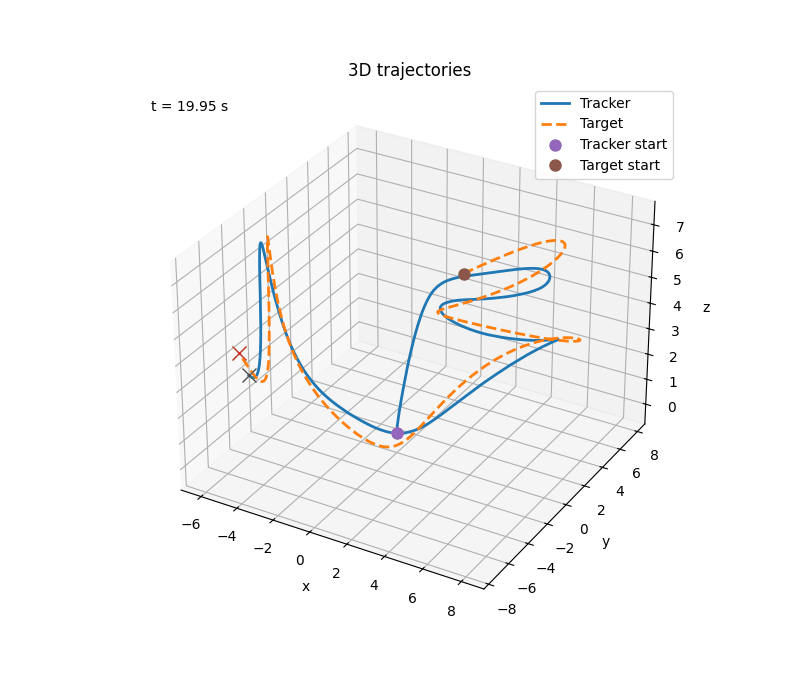
\includegraphics[width=0.75\textwidth]{tracker_target_3d_final.png}
\end{center}
\caption{3D trajectories of the tracker drone (solid blue) and target (dashed orange) at $t = 19.95\,$s. After a short initial transient the tracker closely mirrors the target through the full maneuver.}
\label{fig:3d}
\end{figure}

Figure~\ref{fig:camera} shows the target's position over time in the tracker's body frame, where the origin represents the tracker's own nose and the red circle marks the desired 1-meter standoff boundary. At $t = 0$ the target begins far from the crosshair, and the blue trajectory traces the controller progressively spiraling the target inward. By $t = 19.95\,$s the orange dot rests near the center of the frame, just inside the red circle, indicating that the tracker has successfully locked onto the target drone's position even with noisy signals.
\begin{figure}[htb]
\begin{center}
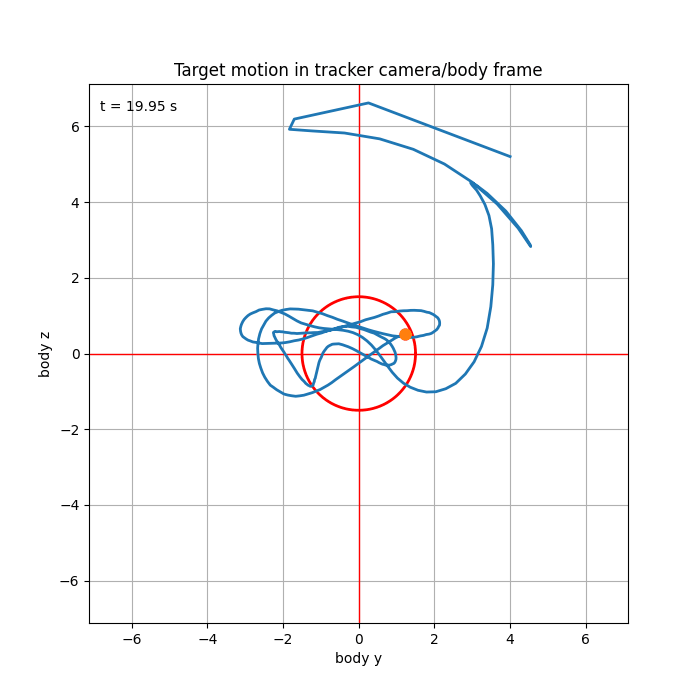
\includegraphics[width=0.75\textwidth]{camera_view_final.png}
\end{center}
\caption{Target position in the tracker's body/camera frame at $t = 19.95\,$s. The blue curve shows the history of the target's apparent position while the orange dot is its final location. The red circle marks the desired 1-meter standoff. The target converges from the upper right toward the desired position.}
\label{fig:camera}
\end{figure}

\FloatBarrier

%%Fourth Section
\section{\textbf{Conclusion}}

The gain-scheduled LQG framework successfully solved the UCAV tracking problem across a wide range of flight conditions. By pre-computing LQR and Kalman filter gains at 27 trim operating points and selecting the nearest at each timestep, the controller maintained close pursuit of an aggressively maneuvering target throughout a 20-second simulation under both process and measurement noise. The 3D trajectory results show that after a brief initial acquisition transient the tracker closely mirrors the target's path, and the camera view results confirm that the 1-meter standoff objective is achieved.

Future work could extend this approach by incorporating rotor saturation constraints more explicitly, exploring nonlinear estimation techniques such as the extended or unscented Kalman filter, and validating the controller on a physical hardware simulator. Increasing the density of the operating-point grid, or replacing the nearest-neighbor scheduler with a smooth interpolation scheme, could further reduce transient switching artifacts and improve performance during rapid flight-regime changes.







%%%%%%%%%%%%%%%%%%%%%%%%%%%%%%%%%%%%%
%% Bibliography below
%%%%%%%%%%%%%%%%%%%%%%%%%%%%%%%%%%%%%
\FloatBarrier % Keep the figures from being put after the bibliography
\newpage
%% If using bibtex, leave this uncommented
\bibliography{refs} %if using bibtex, call your bibtex file refs.bib

\begin{thebibliography}{9}

\bibitem{astrom_murray}
K. J. Åström and R. M. Murray,
\textit{Feedback Systems: An Introduction for Scientists and Engineers},
Princeton University Press, 2008.

\end{thebibliography}

%% If not using bibtex, comment out the previous two lines and uncomment those below
%\begin{thebibliography}{99}
%\bibitem{Vandermeersch} First reference goes here
%\end{thebibliography}

\end{document}
